Encuentra el valor de la incógnita en el triángulo de la figura \ref{fig:angle_triangle_35}.

\begin{minipage}[t][5cm][b]{0.3\textwidth}
    \begin{figure}[H]
        \centering
        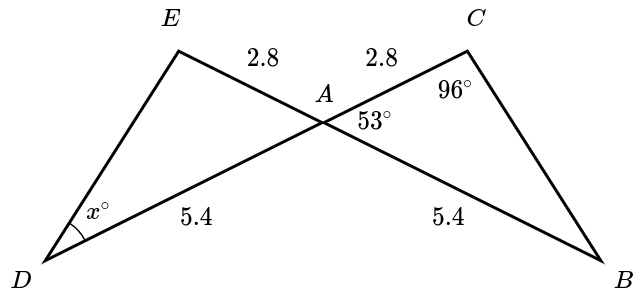
\includegraphics[width=\linewidth]{../images/angle_triangle_35.png}
        \caption{}
        \label{fig:angle_triangle_35}
    \end{figure}
\end{minipage}\hfill
\begin{minipage}[t]{0.65\textwidth}
    \begin{solutionbox}{5cm}
        $\angle DAE$ forma un ángulo opuesto por el vértice con $\angle BAC$, por lo tanto la medida de $\angle DAE$ es igual a la medida de $\angle BAC$.

        $\triangle ABC$ y $\triangle ADE$ también tienen dos lados iguales. Por lo tanto,
        $\triangle ABC$ y $\triangle ADE$ son congruentes.

        Los triángulos congruentes también tienen ángulos congruentes (iguales). Si superponemos estos dos triángulos, volteando $\triangle EDA$, observamos que el ángulo $x$ corresponde al $\angle ABC$.

        $\angle ABC$ mide: \[x=180^\circ-53^\circ-96^\circ=31^\circ\]
    \end{solutionbox}
\end{minipage}
